% Chapter x

\chapter{安全性设计}

\section{生成安全的前端页面}

所有返回给用户的前端页面都经由Thymeleaf模板引擎渲染而成,我们遵照规范,正确的使用了Thymeleaf模板,因此从源头杜绝了所有可能的XSS攻击,包括Stored XSS和Reflected XSS漏洞都不会出现在我们的网站中。下面是一个典型的Thymeleaf模板示例。

\begin{minted}
[
	frame=lines,
	framesep=2mm,
	baselinestretch=1.2,
	bgcolor=lightgray,
	fontsize=\footnotesize,
	linenos
]{html}

<div class="w3-card-4 w3-padding-16 w3-white w3-container" th:if="${has_error}">
     <div class="w3-center">
            <b style="color:red" th:text="${error_msg}"></b>
     </div>
</div>

\end{minted}

\section{校验用户输入}

任何由用户提交给服务器端的信息都有可能成为恶意攻击者的突破口,忽视或不完善的校验检查往往会让恶意攻击者有机可乘。

\subsection{注册表单校验规则}\label{sec:registerV}

\begin{itemize}
	\item \textbf{用户名校验规则}
	
	为保证用户名的强度,我们要求一个合法的用户名必须不少于6个字符,并不多于18个字符。每一个字符都必须是ASCII字母,ASCII数字,或者下划线“\_”。
	
	\item \textbf{密码校验规则}
	
	密码的强度对于一个系统的安全来说至关重要,弱密码如“123456”、“root”、“qwert”都极易被攻击者猜中。因此为保证用户的密码强度,我们要求一个合法的密码必须必须不少于6个字符,并不多于18个字符。每一个字符都必须是可打印出来的ASCII字符。并且整个密码必须同时包含大写字母、小写字母、数字和特殊符号(例如百分号、下划线等)。
	
	\item \textbf{电子邮箱地址校验规则}
	
	我们认为电子邮箱地址应当是一个合法的互联网地址,因此利用了JavaMail中的InternetAddress类来校验它。代码示例如下。
	
\begin{minted}
[
	frame=lines,
	framesep=2mm,
	baselinestretch=1.2,
	bgcolor=lightgray,
	fontsize=\footnotesize,
	linenos
]{java}

public static boolean isValidEmail(String email) {
        try {
                InternetAddress emailAddr = new InternetAddress(email);
                emailAddr.validate();
                return true;
        } catch (AddressException ex) {
                return false;
        }
}

\end{minted}
	
	\item \textbf{重复密码校验规则}
	
	为确保用户输入了其设想中的密码,避免由于键盘误操作带来的错误。我们要求用户输入两次索要设置的密码,只有两次密码完全相同的时候才被认为密码正确,通过校验。
	
\end{itemize}

\subsection{电子邮箱的验证规则}\label{sec:emailV}

用户在刚刚注册完,或者是刚刚更换电子邮箱地址之后。这个新的电子邮箱地址会处于“未验证”的状态。我们估计用户通过我们的系统验证这个电子邮箱地址。当用户在登录后点击个人主页中的“VERIFY YOUR EMAIL ADDRESS”链接后,一封电子邮件会被发送到用户指定的邮箱中,其中会包含一个链接,点击该链接就可以完成对电子邮箱的验证。

\subsection{文件上传的验证规则}\label{sec:fileV}

文件的上传在网络生活中及其常见,应用广泛。但往往不严谨的实现会留下安全隐患,给恶意攻击者留下攻击服务器的空间。我们在这里进行了多次验证,主要防范了以下的潜在攻击方式
\begin{itemize}

	\item \textbf{耗尽服务器资源的攻击}
	
	为了防止服务器的磁盘资源被恶意攻击者用很多大文件抢占一空,我们限制了单个上传的文件大小上限,现阶段我们只允许上传小于10MB的文件。
	
	\item \textbf{恶意文件名攻击}
	
	恶意攻击者有可能会上传形如“../../file.txt”的文件,使得该文件有可能会存储在服务器指定的存储根目录外,造成未知的、及其难以排查的错误。因此我们会仔细检查文件名,拒绝所有包含路径分隔符的非法文件名。
	
	\item \textbf{恶意程序注入}
	
	恶意攻击者有可能会上传包含恶意程序的代码片段,并试图通过别的手段让这段代码在服务器端运行,从而制造后门或或获取更大的服务器权限。因此我们采取文件拓展名白名单的形式限制了可以上传的文件类型。只有形如以下拓展名的文件才能被成功上传:
	\begin{itemize}
		\item \textbf{文档类}
		
		docx,doc,pptx,ppt,xlsx,xls,pdf
		
		\item \textbf{图片类}
		
		jpeg,jpg,png,gif,tiff,tif,raw,bmp,svg
		
		\item \textbf{纯文本类}
		
		txt,tex,md
		
		\item \textbf{音频类}
		
		mp3,wav
		
		\item \textbf{压缩类}
		
		zip,z,rar,7z,gz,tar
		
		\item \textbf{数据类型}
		
		csv,xml
	\end{itemize}

\end{itemize}

\section{Session安全分析}\label{sec:sessionS}

我们为用户生成的的Cookie是长达16字节的随机数。16个字节总共会包含128个比特,即一共会有$2^{128}$种可能的排列组合。这个取值空间是如此之大,基本上可以近似于认为我们的Session是永远不会重复的,没有重用的风险。同时Session会有有效时间的限制,如果用户在30分钟内没有进行任何操作的话,用户的Session将会过期,需要重新登录。

\section{处理错误和异常}

由于未被catch的exception,或者其他种种难以预料到的情形,服务器常常会产生错误的响应。这类错误信息如果未经处理是及其危险的,因为往往默认的做法是打印stack trace(如图\ref{fig:stacktrace})。这样的暴露是及其危险的,其中很有可能会泄露部分代码细节,从而让恶意攻击者找到下一步攻击服务器的突破口,进而带来更大的恶劣影响。在本项目中,我们统一编写了一个用于在异常情况下响应的控制器,该控制器会返回我们自己设计的统一风格的错误界面,在保证整体网站风格统一的前提下,隐藏了所有可能会暴露代码细节的信息。

\begin{figure}[!htb]
	\centering
	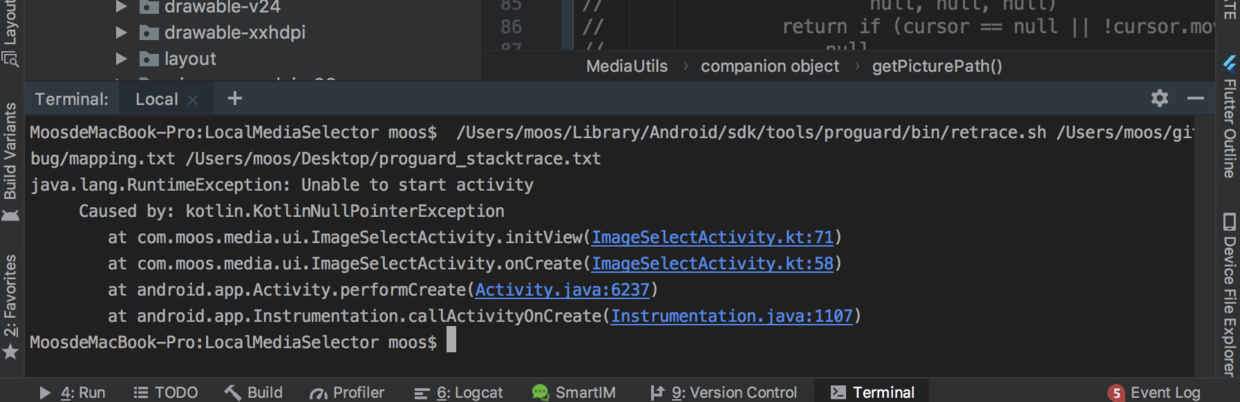
\includegraphics[width=0.8\textwidth]
	{figures/stacktrace.jpg}\\
	\caption{可能会暴露代码细节信息的stack trace}
	\label{fig:stacktrace}
\end{figure}


